\documentclass[tikz,border=10pt]{standalone}
% No extra TikZ libraries needed.
\begin{document}
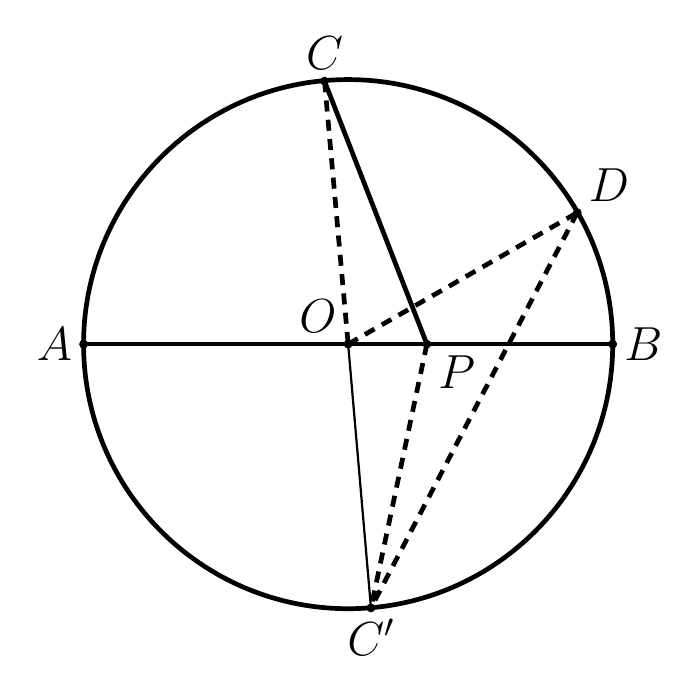
\begin{tikzpicture}[line join=round, line width=1.7pt]
  % Scale s = 0.021333 cm/px (from STYLE METRICS); centre = circle centre (224.2, 222.0) px
  \coordinate (O) at (0,0);
  \coordinate (A) at (-3.36,0);
  \coordinate (B) at (3.36,0);
  \coordinate (C) at (-0.30,3.34);
  \coordinate (Cp) at (0.29,-3.35);
  \coordinate (D) at (2.91,1.67);
  \coordinate (P) at (1.00,0);

  % Circle (thick, black)
  \draw (O) circle[radius=3.36];

  % Solid segments
  \draw (A) -- (B);                    % diameter AB
  \draw (C) -- (P);                    % CP
  \draw[line width=0.8pt] (O) -- (Cp); % OC' thin solid

  % Dashed segments (explicit dash pattern, not dotted)
  \draw[dash pattern=on 4pt off 3pt] (C) -- (O);   % CO
  \draw[dash pattern=on 4pt off 3pt] (O) -- (D);   % OD
  \draw[dash pattern=on 4pt off 3pt] (D) -- (Cp);  % DC'
  \draw[dash pattern=on 4pt off 3pt] (P) -- (Cp);  % PC'

  % Small filled dots
  \foreach \X in {A,B,C,Cp,D,O,P}
    \fill (\X) circle[radius=1.6pt];

  % Labels (font from cap-height metrics)
  \begin{scope}[font=\fontsize{18}{21.6}\selectfont]
    \node[left]        at (A)  {$A$};
    \node[right]       at (B)  {$B$};
    \node[above]       at (C)  {$C$};
    \node[above right] at (D)  {$D$};
    \node[above left]  at (O)  {$O$};
    \node[below right] at (P)  {$P$};
    \node[below]       at (Cp) {$C'$};
  \end{scope}
\end{tikzpicture}
\end{document}